\documentclass[xcolor=svgnames]{beamer}

\usepackage{bera}
\usepackage[utf8]    {inputenc}
\usepackage[T1]      {fontenc}
\usepackage[english] {babel}

\usepackage{amsmath,amsfonts,graphicx}
\usepackage{beamerleanprogress}

\title
	[Escalabilidad de SDN en la RAU]
  {Proyecto de grado \\
  	Escalabilidad de Redes Definidas por Software en la Red Académica}

\author
	[Santiago Vidal]
  {Santiago Vidal \\
  	\vspace{4mm}
  	{\normalfont\small Tutores: \\
  	Dr. Eduardo Grampín \\
  	MSc. Martín Giachino}}

\date
  {5 de octubre de 2016}

\institute
  [UdelaR]
  {Instituto de Computación \\
  	Facultad de Ingeniería \\
  	Universidad de la República}


\begin{document}

% Directorio con las imagenes
\graphicspath{{Figs/}}

\maketitle

\begin{frame}{}
	\tableofcontents
\end{frame}

\section{Introducción}

\begin{frame}
	\tableofcontents[currentsection]
\end{frame}

\begin{frame}{Introducción}
	\begin{block}{Red Académica Uruguaya (RAU)}
		\begin{itemize}
			\item Emprendimiento de la Universidad de la República, administrado por el Servicio Central de Informática Universitario
			(SeCIU).
			\item Red que conecta instituciones académicas, centros de investigación e instituciones gubernamentales.
		\end{itemize}
	\end{block}
	\begin{block}{RAU2}
		RAU2 es un proyecto para reemplazar la infraestructura actual, con el objetivo de brindar más y mejores servicios a las instituciones.
	\end{block}
\end{frame}
%La idea de esta red es proveer servicios especializados para las insituciones, mayor calidad de servicio, mas velocidad, etc.
%Proveedores sobrevenden ancho de banda
%Actividades comerciales y particulares tienen misma prioridad.

\begin{frame}{Proyecto RRAP}
	\textbf{Routers Reconfigurables de Altas Prestaciones} (Emiliano Viotti, Rodrigo Amaro):
	\begin{itemize}
		\item Proyecto de grado que terminó en agosto de 2015.
		\item Desarrolló una arquitectura de red basada en SDN llamada \textbf{RAUFlow}, que implementa Redes Privadas Virtuales (VPN).
		\item Construyó un prototipo físico para validación funcional.
	\end{itemize}
\end{frame}

\begin{frame}{Proyecto RRAP}
	\begin{center}
		Prototipo físico para pruebas funcionales:
		\begin{figure}[t]
			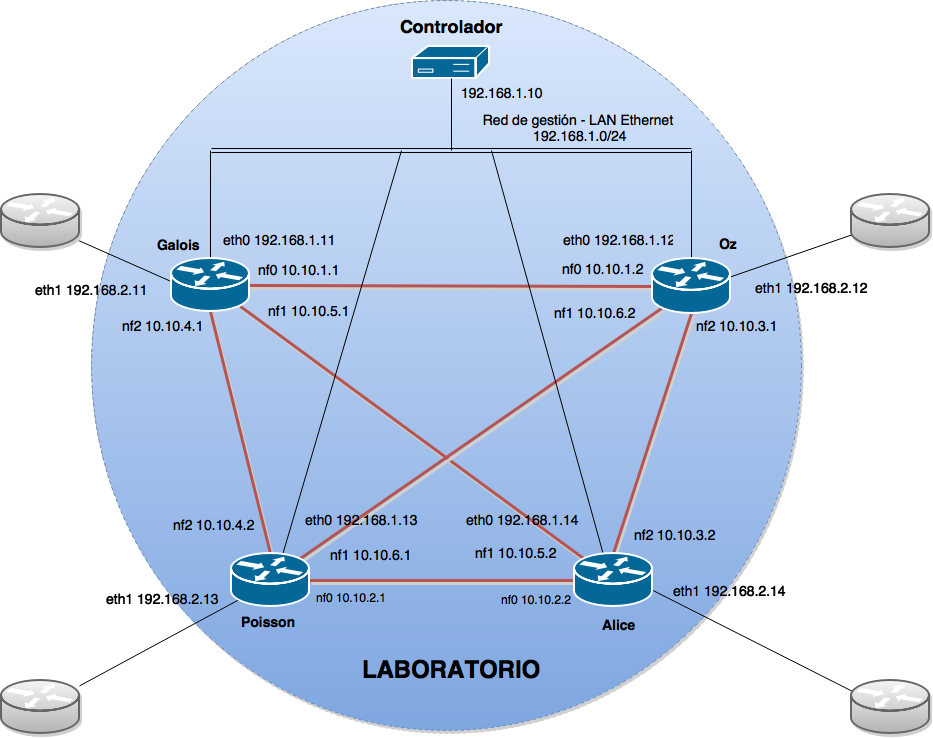
\includegraphics[scale=0.25]{topologia_rrap}
		\end{figure}
	\end{center}
\end{frame}

\begin{frame}{Motivación}
	Contestar las siguientes preguntas:
	\pause
	\begin{enumerate}
		\item ¿Cómo podemos seguir trabajando sobre la arquitectura RAUflow sin ser limitados por el prototipo físico?
		\pause
		\item ¿RAUFlow funciona con topologias más grandes?
		\pause
		\item ¿Tiene buena escalabilidad?
		%Por qué es importante estudiar la escalabilidad?
	\end{enumerate}
\end{frame}

\begin{frame}{Resultados esperados}
	\pause
	\begin{enumerate}
		\item Una \textbf{herramienta} que permita virtualizar la arquitectura RAUFlow para pruebas y desarrollo.
		\pause
		\item Diseño e implementación de \textbf{pruebas} para estudiar la escalabilidad de RAUFlow.
	\end{enumerate}
\end{frame}

\section{Conceptos previos \& RAUFlow}

\begin{frame}{}
	\tableofcontents[currentsection]
\end{frame}

\begin{frame}{Conceptos previos}
	Estudiemos algunos conceptos previos relacionados a RAUFlow:
	\begin{enumerate}
		\item VPN
		\item MPLS
		\item Software Defined Networking
		\item OpenFlow
	\end{enumerate}
\end{frame}

\begin{frame}{VPN}
	Red privada que se extiende a través de una red pública, como Internet. Puede ser de capa 2 (enlace) o 3 (red) del modelo OSI.
	\begin{center}
		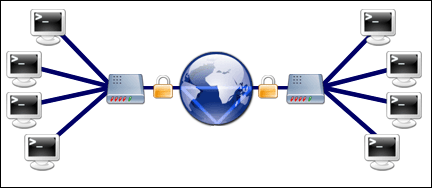
\includegraphics[scale=0.8]{vpn}
	\end{center}
\end{frame}

\begin{frame}{MPLS}
	Mecanismo de transporte de datos basado en la conmutación de etiquetas. Es la solución de facto para la implementación de servicios de VPN.
	\begin{center}
		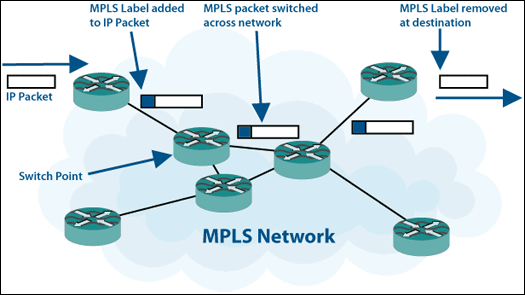
\includegraphics[scale=0.6]{mpls}
	\end{center}
\end{frame}

\begin{frame}{Redes Definidas por Software (SDN)}
	\begin{figure}[t]
		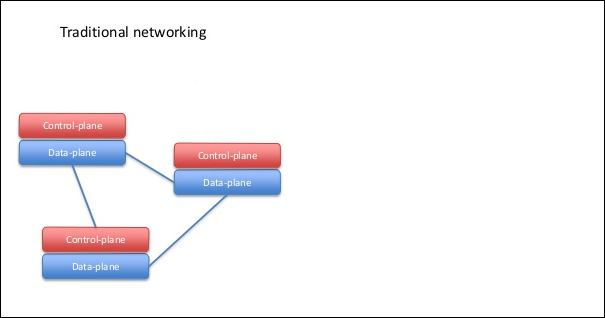
\includegraphics[scale=0.6]{sdn_transicion1}
	\end{figure}
\end{frame}

\begin{frame}{Redes Definidas por Software (SDN)}
	\begin{figure}[t]
		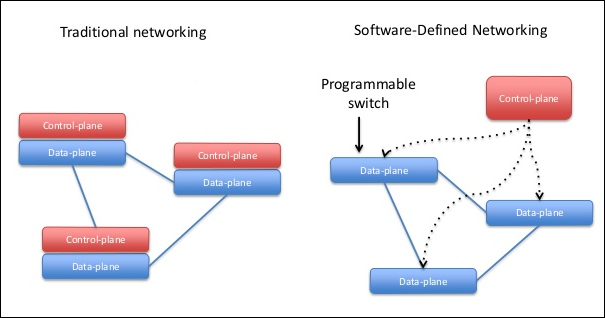
\includegraphics[scale=0.6]{sdn_transicion}
	\end{figure}
\end{frame}

\begin{frame}{Redes Definidas por Software (SDN)}
	\begin{figure}[t]
		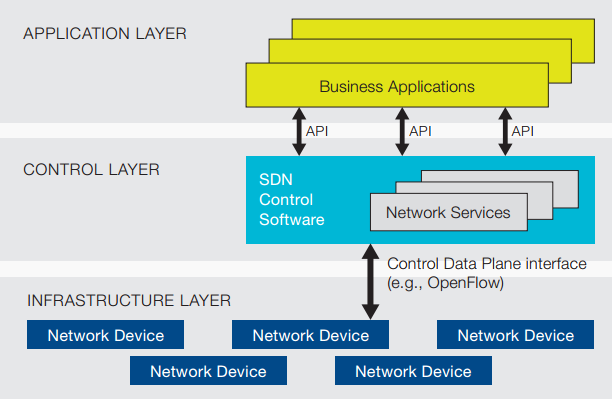
\includegraphics[scale=0.6]{arquitectura_sdn}
	\end{figure}
\end{frame}
%Empezar desde abajo
%Decir ejemplo DDOS

\begin{frame}{OpenFlow}
	\begin{itemize}
		\item Provee una forma de abstraer las capacidades de un dispositivo.
		\item Protocolo de comunicación con el controlador OpenFlow.
	\end{itemize}
	\pause
	\vspace{4mm}
	\begin{center}
		Flujo OpenFlow: \\
		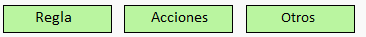
\includegraphics[scale=0.7]{flujo_openflow}
	\end{center}
	\begin{itemize}
		\item Regla: Define el tipo de tráfico.
		\item Acciones: Define qué se debe hacer con los paquetes del flujo (Drop, Output, Agregar/Quitar etiqueta MPLS)
		\item Otros: Estadísticas, Prioridad, Timeout, etc.
	\end{itemize}
\end{frame}

\begin{frame}{RAUFlow}
	Aplicación para control de red basada en el controlador Ryu.
	\begin{enumerate}
		\item Implementa servicios de VPN de capa 2 y 3.
		\item OpenFlow y MPLS.
		\item OSPF y SNMP.
	\end{enumerate}
	\begin{minipage}[b]{0.4\textwidth}
		\begin{center}
			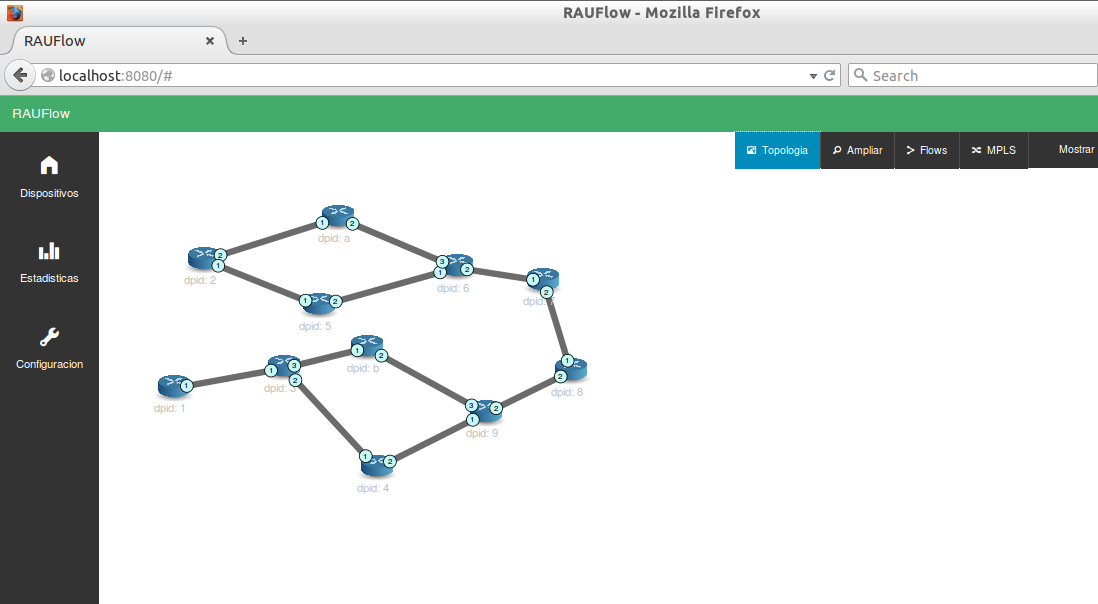
\includegraphics[scale=0.20]{rauflow_interfaz2}
		\end{center}
	\end{minipage}
	\hfill
	\begin{minipage}[b]{0.4\textwidth}
		\begin{center}
			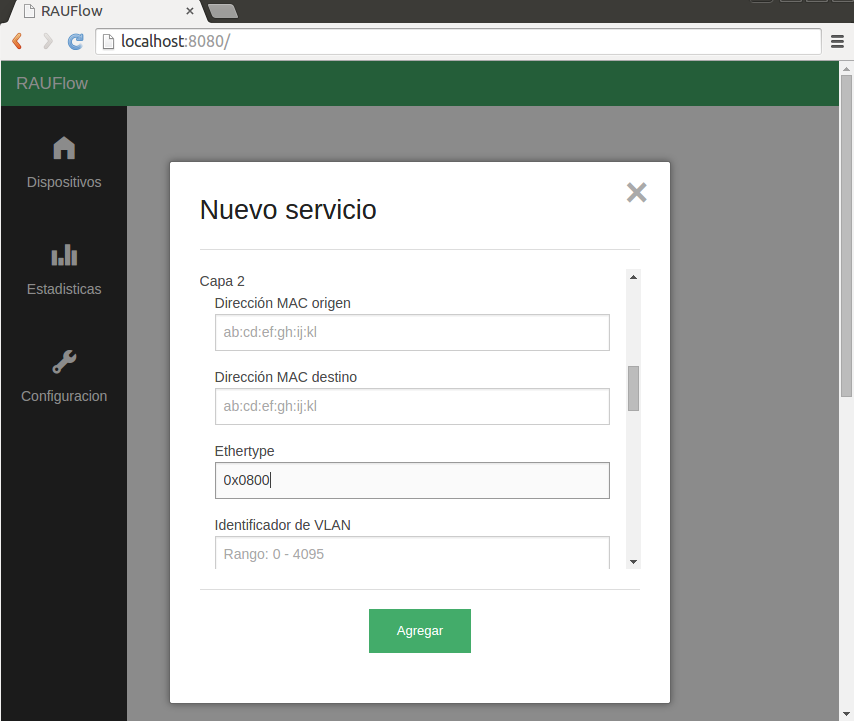
\includegraphics[scale=0.20]{rauflow_interfaz}
		\end{center}
	\end{minipage}
\end{frame}

\begin{frame}{RAUFlow}
	\begin{center}
		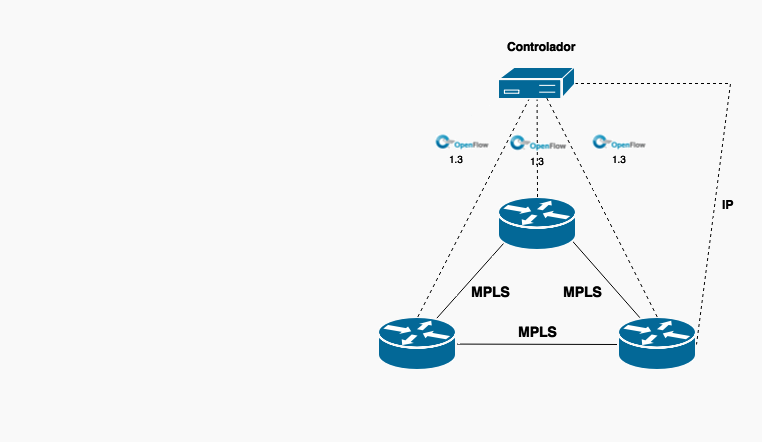
\includegraphics[scale=0.6]{componentes_rauflow01}
	\end{center}
\end{frame}

\begin{frame}{RAUFlow}
	\begin{center}
		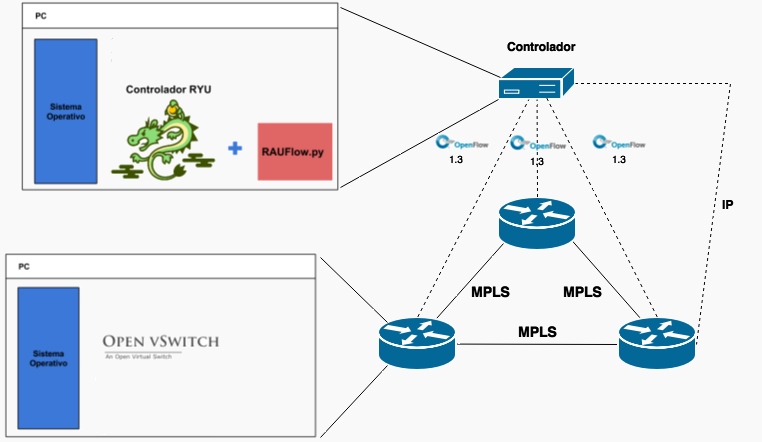
\includegraphics[scale=0.6]{componentes_rauflow02}
	\end{center}
\end{frame}

\begin{frame}{RAUFlow}
	\begin{center}
		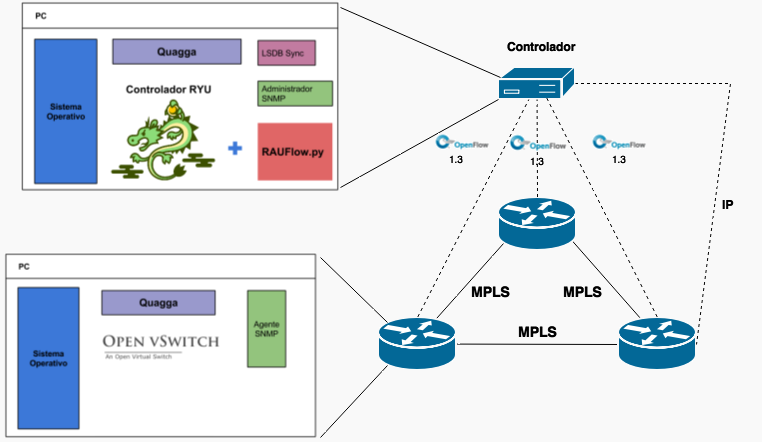
\includegraphics[scale=0.6]{componentes_rauflow}
	\end{center}
\end{frame}

\section{Entorno virtual}

\begin{frame}{}
	\tableofcontents[currentsection]
\end{frame}

\begin{frame}{Objetivo}
	Poder utilizar la arquitectura RAUFlow y RAUSwitch en un entorno virtual para:
	\begin{itemize}
		\item Experimentos y pruebas.
		\item Desarrollo de nuevas funcionalidades sobre RAUFlow.
	\end{itemize}
\end{frame}
%Pruebas y experimentos que no son posibles con prototipos físicos. Incluso si se contara con todo el equipamiento, la configuración es muy compleja.

\begin{frame}{Requerimientos}
	Requerimientos funcionales:
	\begin{enumerate}
		\item RAUSwitch virtuales:
		\begin{enumerate}
			\item OpenFlow 1.3
			\item OSPF
			\item SNMP (no esencial)
		\end{enumerate}
		\item Hosts virtuales
		\item Controlador RAUFlow
	\end{enumerate}
	\pause
	Requerimientos no funcionales:
	\begin{enumerate}
		\item Configurabilidad / Usabilidad
		\item Escalabilidad
	\end{enumerate}
\end{frame}

\begin{frame}{Siguiente paso}
	\begin{center}
		Se descarta una construcción desde cero
	\begin{figure}[t]
		
\includegraphics[scale=0.1]{arrow_down}
	\end{figure}
	Hay que encontrar una herramienta que cumpla los requerimientos
	\end{center}
\end{frame}

\begin{frame}{Elección de una herramienta}
	\begin{alertblock}{Herramientas orientadas a SDN}
		\begin{itemize}
			\item Algunas no soportan OpenFlow 1.3
			\item Algunas no permiten un controlador externo.
			\item \textbf{Ninguna contempla switches híbridos!}
		\end{itemize}
	\end{alertblock}
	\pause
	\begin{block}{Herramientas de propósito general}
		\begin{itemize}
			\item Algunas no tienen buena configurabilidad.
			\item La \textbf{escalabilidad} es un gran problema.
		\end{itemize}
	\end{block}
\end{frame}

\begin{frame}{Mininet}
	\begin{itemize}
		\item Emulador de redes.
		\item Comúnmente utilizado para experimentar con SDN y OpenFlow.
		\item Ofrece Hosts y Switches.
		\item Virtualización ligera (containers).
		\item Cumple todos los requerimientos \textbf{excepto} el soporte para switches híbridos.
		\item Permite al usuario definir sus propias clases de nodos para extender las funcionalidades de las clases que vienen por defecto.
	\end{itemize}
\end{frame}

\begin{frame}{Arquitectura de Mininet}
	\begin{figure}[t]
		\centering
		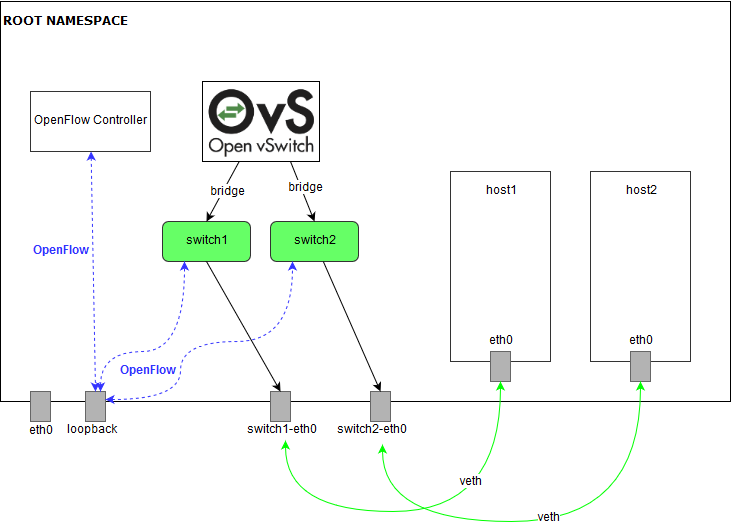
\includegraphics[scale=0.5]{mininet_architecture}
	\end{figure}
\end{frame}
% Los recursos de red de cada switch no están aislados entre sí.

\begin{frame}{Problema con Mininet tradicional}
	\begin{itemize}
		\item Los switches están en el root namespace, así que no es posible que cada uno ejecute su instancia de Quagga.
		\item No es posible poner a cada Switch en su propio namespace ya que Open vSwitch no tendría acceso a ellos.
		\item Si los switches están en su propio namespace, el controlador OpenFlow (RAUFlow) no puede comunicarse con ellos a través de la interfaz de loopback.
	\end{itemize}
	\pause
	{\color{teal}Solución: utilizar Mininet pero como emulador de propósito general.}
\end{frame}

\begin{frame}{Diseño de la solución}
	\begin{figure}[t]
		\centering
		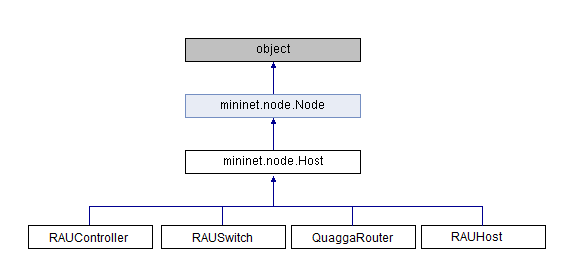
\includegraphics[scale=0.7]{clases_entorno}
	\end{figure}
\end{frame}

\begin{frame}{Arquitectura del entorno construido}
	\begin{figure}[t]
		\centering
		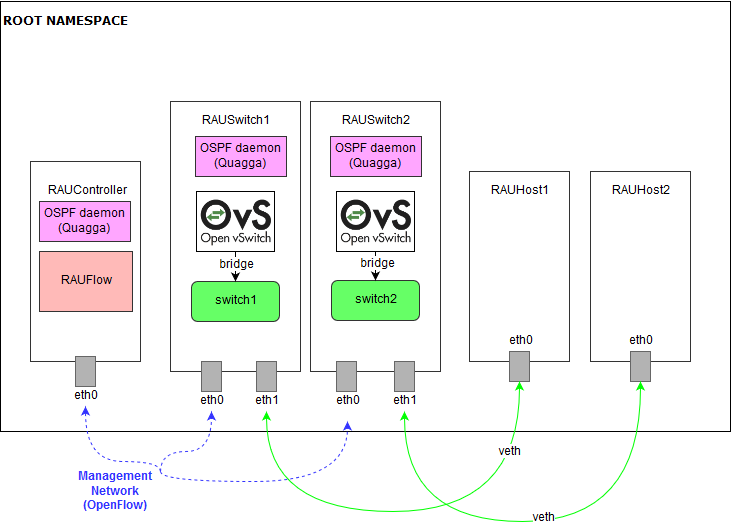
\includegraphics[scale=0.5]{emulator_architecture}
	\end{figure}
\end{frame}
%Aca mencionar que OVS es el aspecto mas radical, y que resulta complejo ejecutar multiples instancias correctamente (capaz mencionar que es gracias a privateDirs, capaz).

\begin{frame}{GraphML Loader}
	\begin{center}
		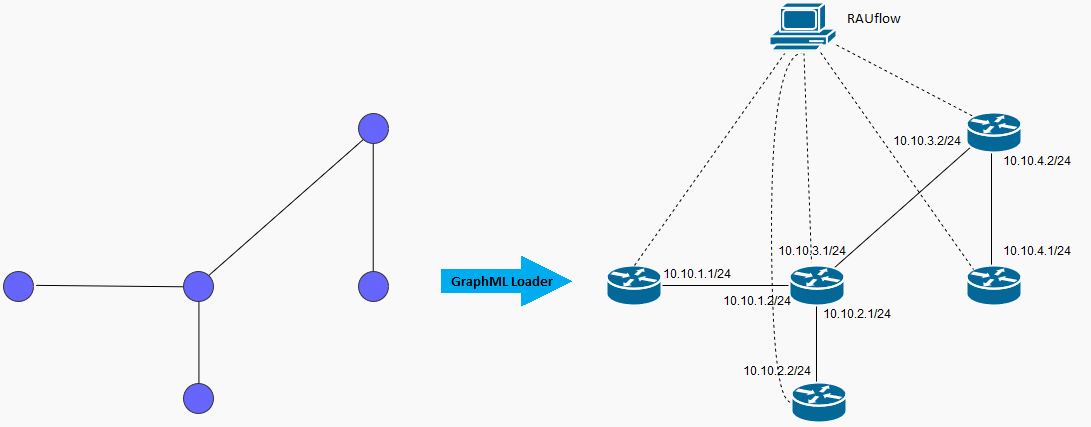
\includegraphics[scale=0.4]{loader}
	\end{center}
\end{frame}

\begin{frame}{Verificación funcional}
	Con el entorno construido, el siguiente paso es probar distintos escenarios y topologias para detectar:
	\begin{itemize}
		\item Problemas con el entorno virtual.
		\item Problemas con la arquitectura/código de RAUFlow.
	\end{itemize}
\end{frame}

\begin{frame}{Problemas encontrados}
	\begin{enumerate}
		\item \textbf{Error en el código de RAUFlow}: error en el algoritmo del camino óptimo. Provocaba una excepción de Python.
		\item \textbf{Error en el código de RAUFlow}: error en el código que instala los flujos OpenFlow en los nodos. Provocaba que los flujos en cada nodo de un camino tuvieran incorrecto puerto de entrada.
	\end{enumerate}
\end{frame}

\begin{frame}{Eliminación de SNMP}
	\begin{figure}[t]
		\centering
		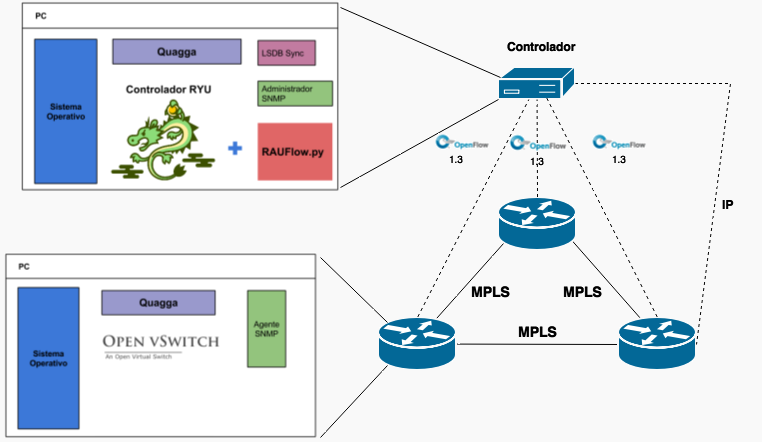
\includegraphics[scale=0.5]{componentes_rauflow}
	\end{figure}
\end{frame}

\begin{frame}{Eliminación de SNMP}
	\begin{figure}[t]
		\centering
		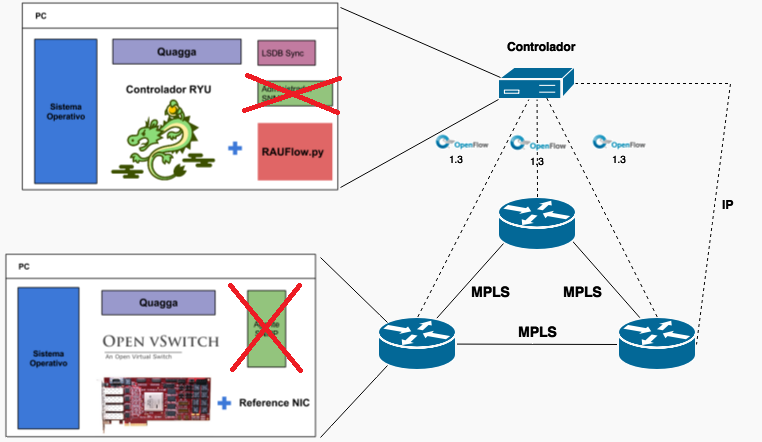
\includegraphics[scale=0.5]{componentes_rauflow_2}
	\end{figure}
\end{frame}

\begin{frame}{Eliminación de SNMP}
	El envío de datos de las interfaces pasa a implementarse con Open vSwitch (por fuera de OpenFlow).
	\begin{exampleblock}{Ventajas}
		\begin{itemize}
			\item Reduce complejidad de la arquitectura.
			\item Reduce carga de cómputo en los switches.
		\end{itemize}
	\end{exampleblock}
\end{frame}

\section{Pruebas de escala}

\begin{frame}{}
	\tableofcontents[currentsection]
\end{frame}

\begin{frame}{Pruebas de escala}
	Podemos analizar la escalabilidad desde dos frentes:
	\begin{enumerate}
		\item \textbf{Variable}: Tamaño de la topología \\
		\textbf{Analizar}: Creación de los servicios
		\item \textbf{Variable}: Nivel de carga \\
		\textbf{Analizar}: Rendimiento de la red \\
	\end{enumerate}
	\pause
	\vspace{4mm}
	\textbf{Observación}: las pruebas no nos dirán valores reales, pero sí nos permiten detectar comportamientos y tendencias.
\end{frame}

\begin{frame}{Pruebas de escala: topologias}
	\begin{minipage}[b]{0.3\textwidth}
		\begin{center}
			Topología básica (prototipo)
			\includegraphics[scale=0.4]{basic_topology}
		\end{center}
	\end{minipage}
	\hfill
	\begin{minipage}[b]{0.6\textwidth}
		\begin{center}
			Topología chica (11 nodos)
			\includegraphics[scale=0.25]{small_topology}
		\end{center}
	\end{minipage}
\end{frame}

\begin{frame}{Pruebas de escala: topologias}
	\begin{center}
		Topología mediana (45 nodos)
		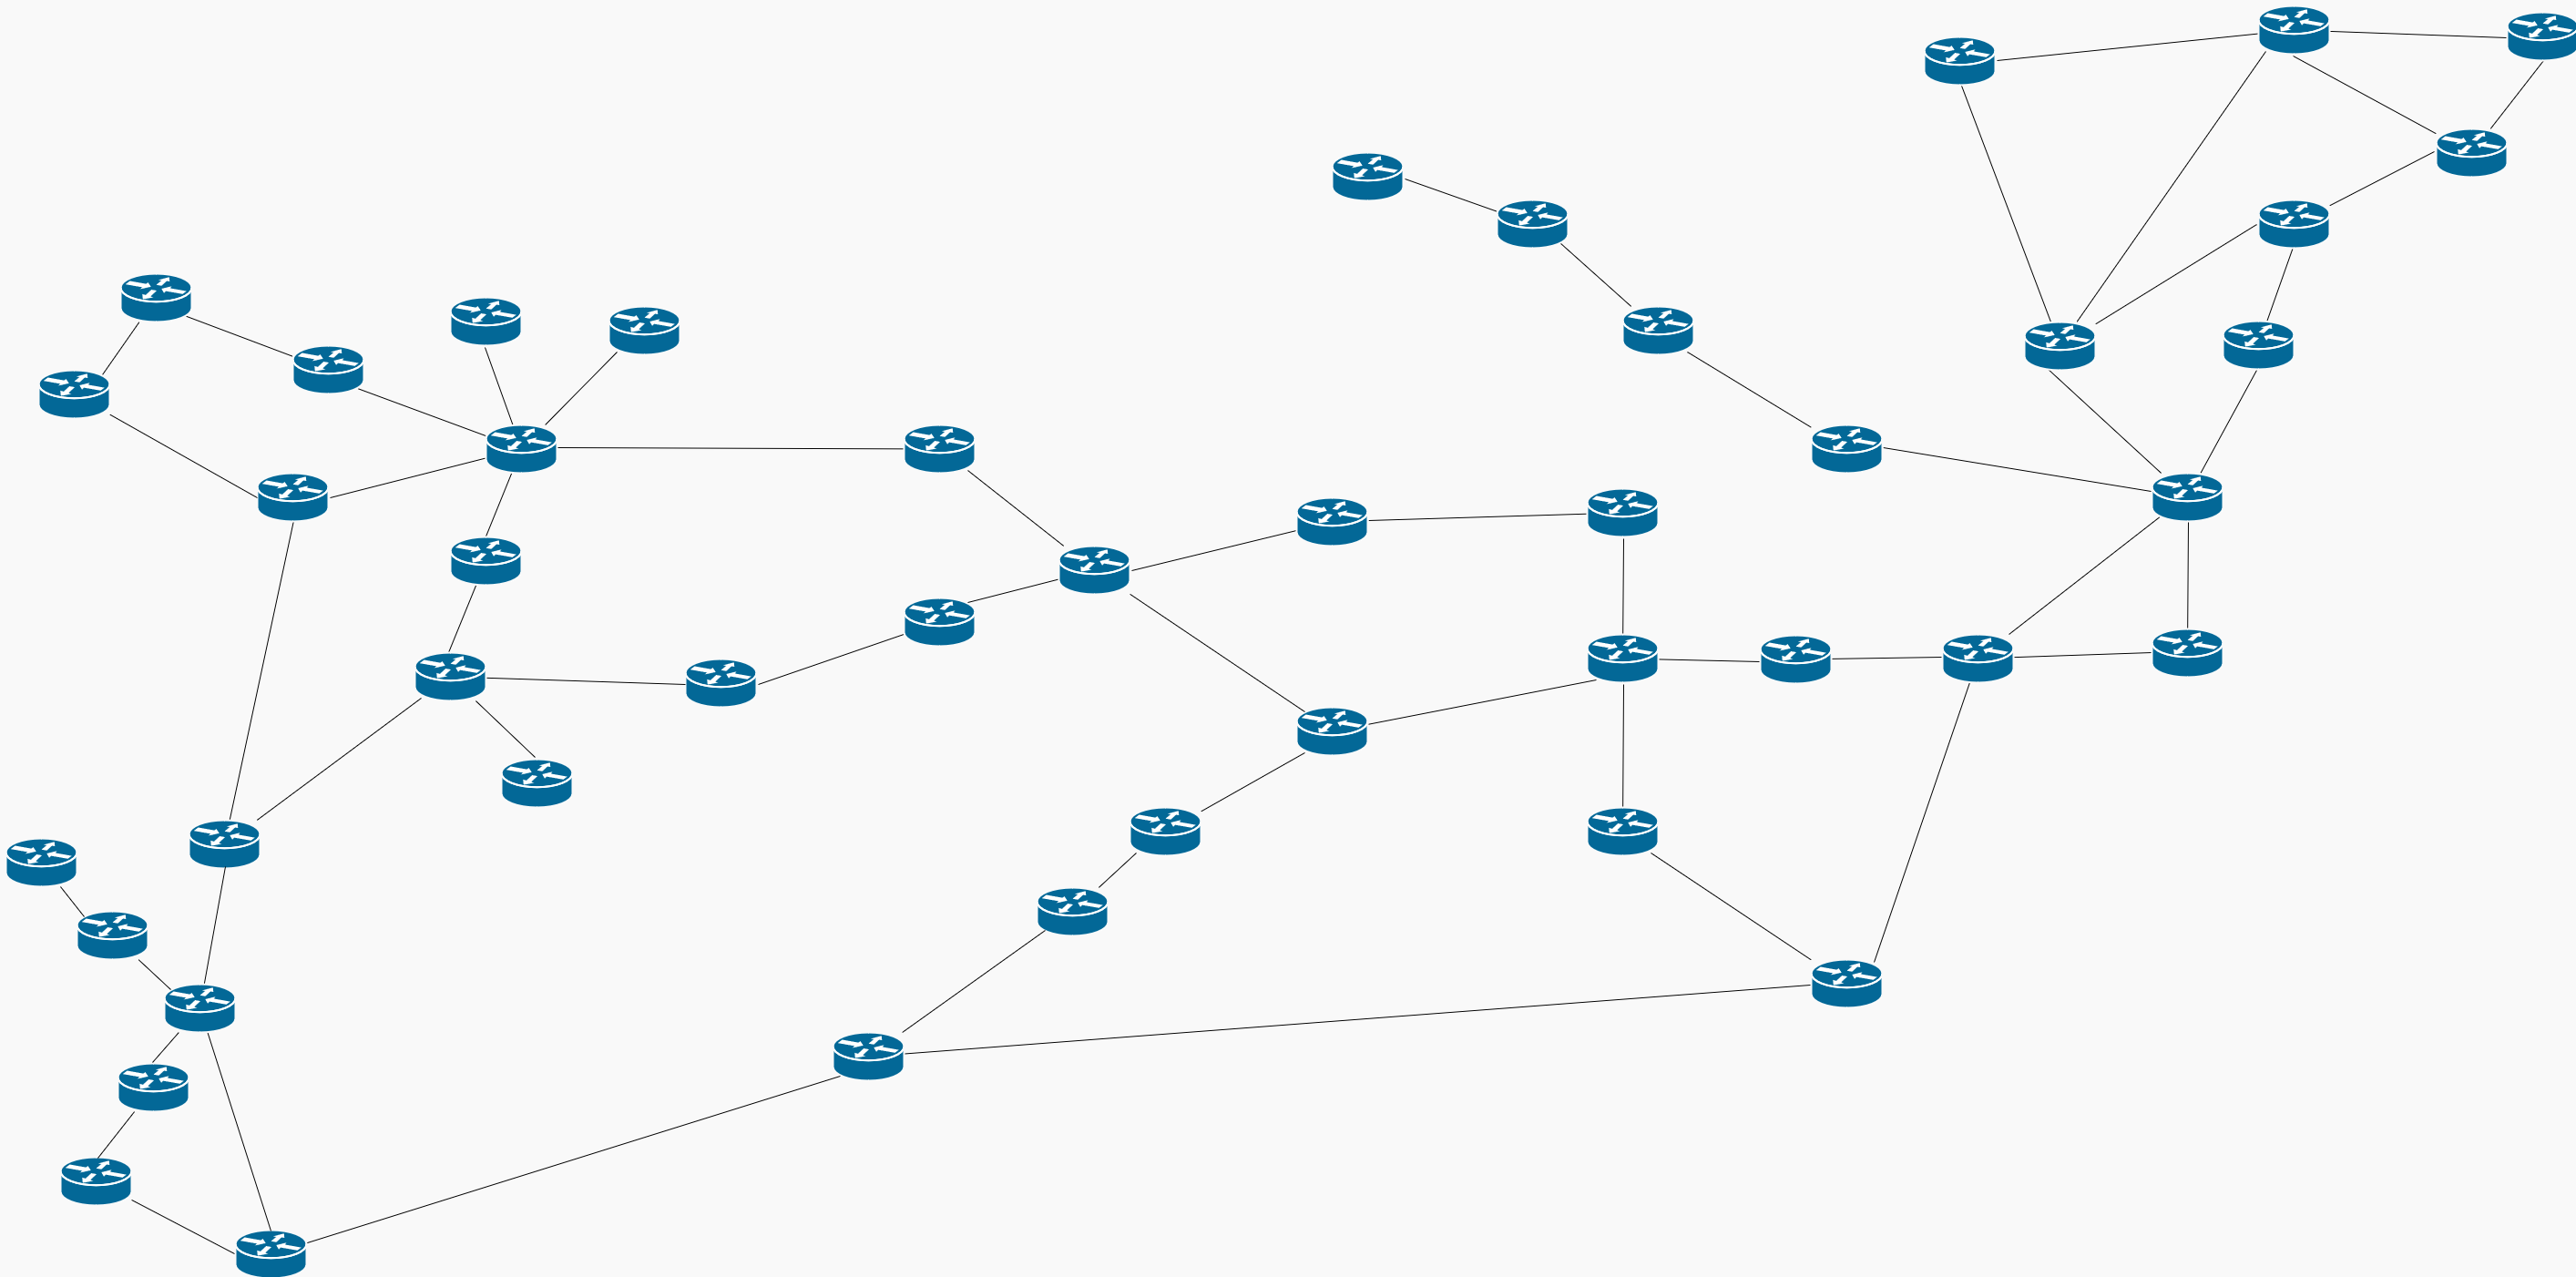
\includegraphics[scale=0.15]{medium_topology}
	\end{center}
\end{frame}

\begin{frame}{Pruebas de escala: topologias}
	\begin{center}
		Topología grande (105 nodos)
		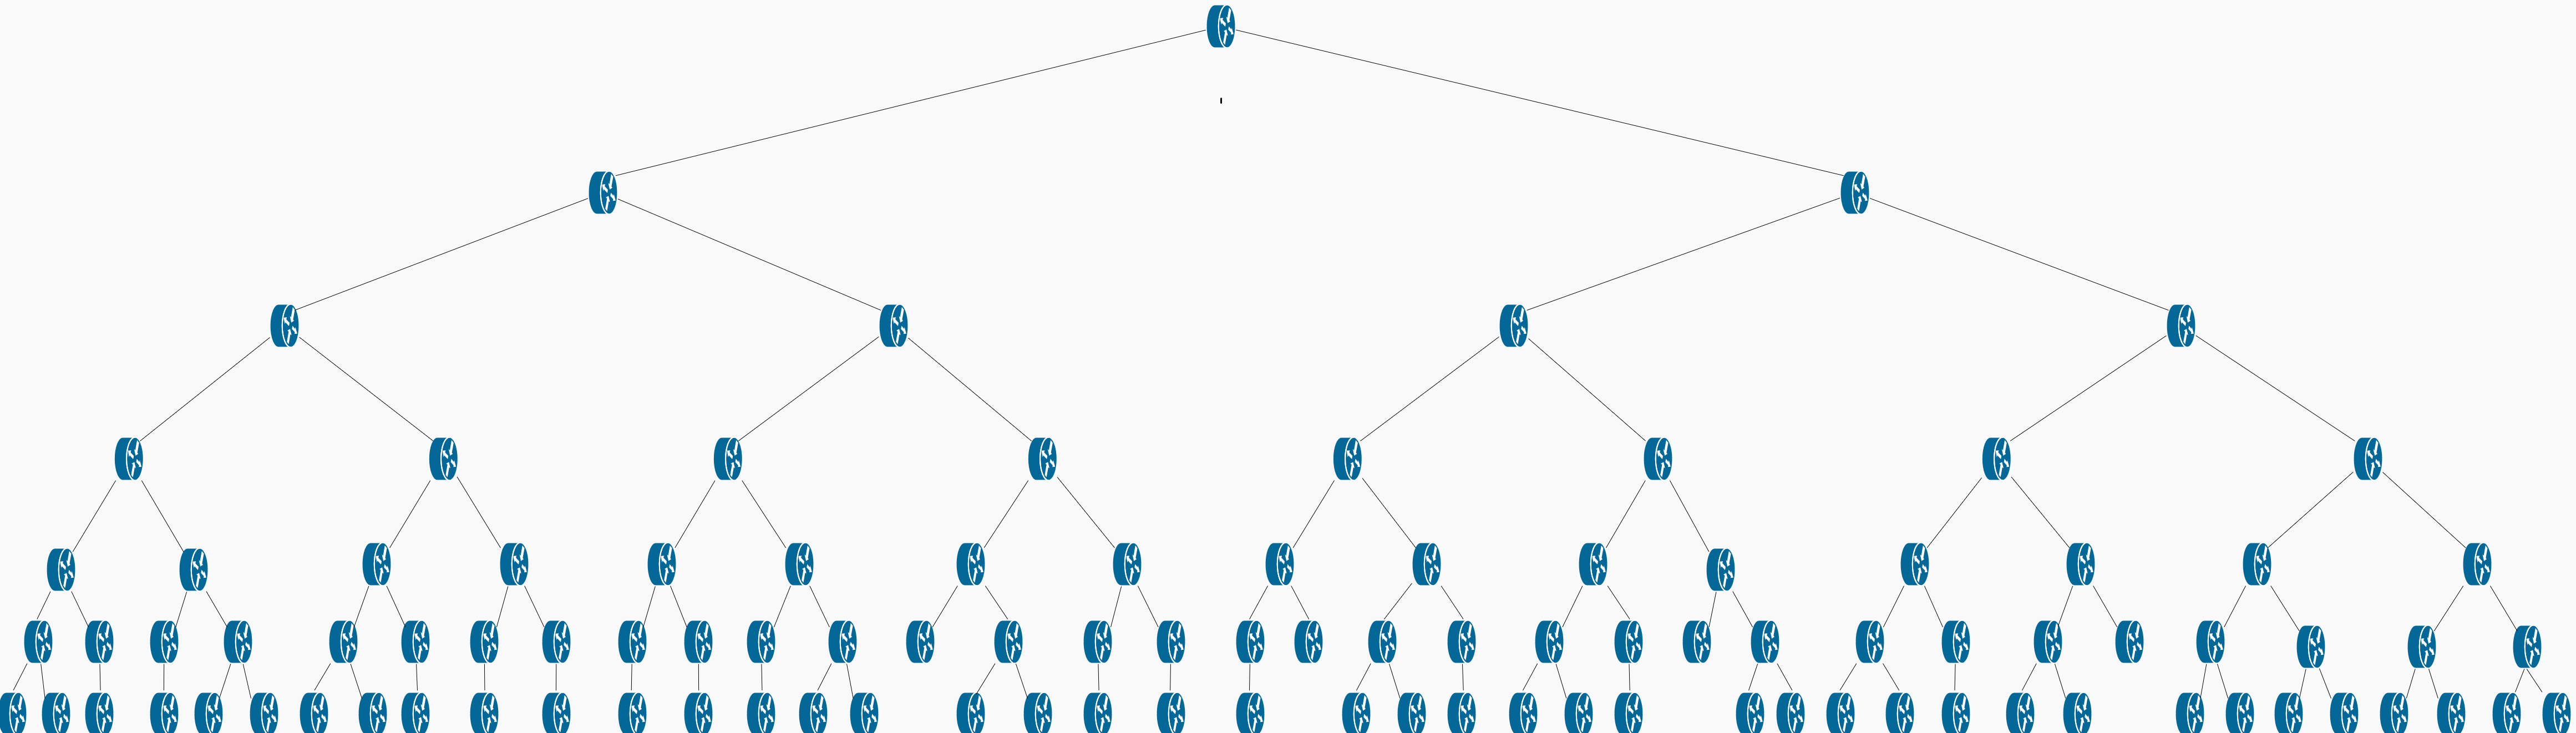
\includegraphics[scale=0.09]{large_topology}
	\end{center}
\end{frame}

\begin{frame}{Tiempos de creación de VPN}
	\begin{center}
		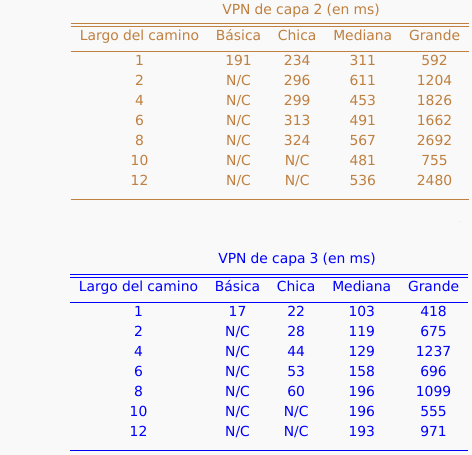
\includegraphics[height=0.9\textheight]{tiempos_vpn}
	\end{center}
\end{frame}

\begin{frame}{Tiempos de creación de VPN}
	\begin{center}
		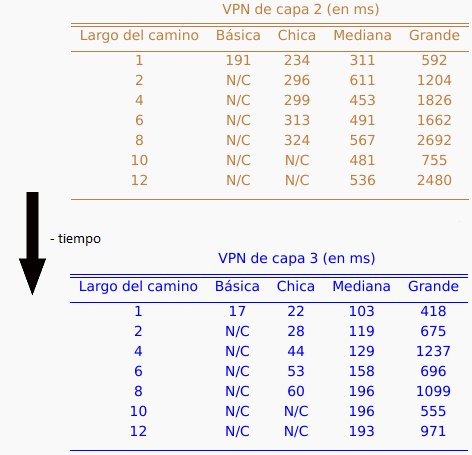
\includegraphics[height=0.9\textheight]{tiempos_vpn_tipo}
	\end{center}
\end{frame}

\begin{frame}{Tiempos de creación de VPN}
	\begin{center}
		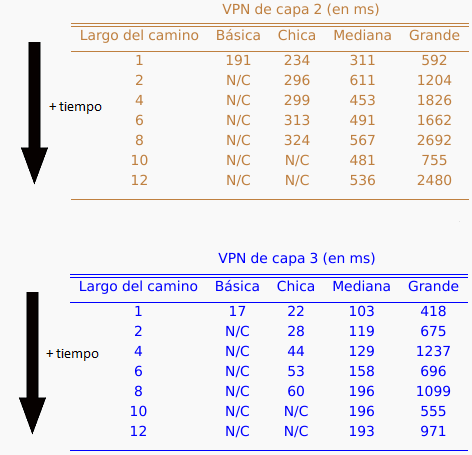
\includegraphics[height=0.9\textheight]{tiempos_vpn_camino}
	\end{center}
\end{frame}

\begin{frame}{Tiempos de creación de VPN}
	\begin{center}
		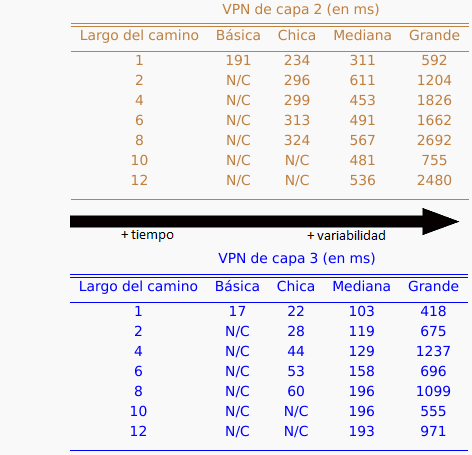
\includegraphics[height=0.9\textheight]{tiempos_vpn_topologia}
	\end{center}
\end{frame}

\begin{frame}{Tiempos de creación de VPN}
	Hagamos un análisis más fino. \\
	\vspace{4mm}
	Agregando \textbf{timestamps} al código podemos ver cuánto tiempo dedica RAUflow a cada tarea:
	\begin{itemize}
		\item Cálculo del camino óptimo
		\item Manejo de etiquetas MPLS
		\item Instalación de flujos OpenFlow
	\end{itemize}
\end{frame}

\begin{frame}{Descomposición del tiempo de creación}
	Topología chica:
	\begin{center}
		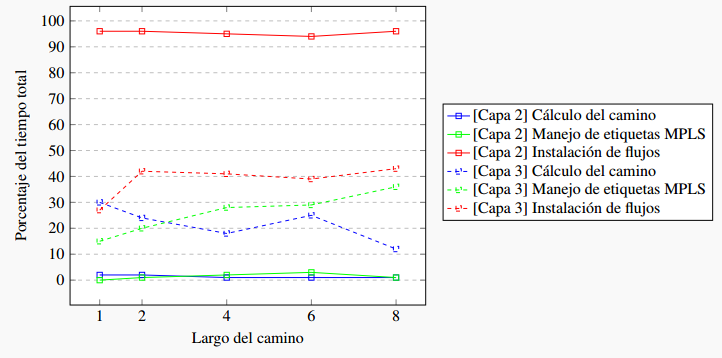
\includegraphics[scale=0.6]{porcentajes_tiempos_chica}
	\end{center}
\end{frame}

\begin{frame}{Descomposición del tiempo de creación}
	Topología mediana:
	\begin{center}
		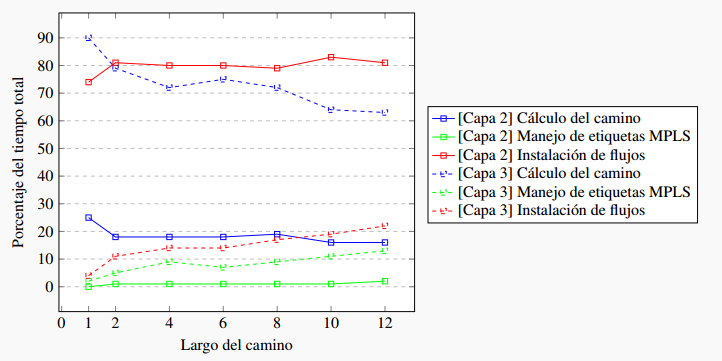
\includegraphics[scale=0.6]{porcentajes_tiempos_mediana}
	\end{center}
\end{frame}

\begin{frame}{Descomposición del tiempo de creación}
	Topología grande:
	\begin{center}
		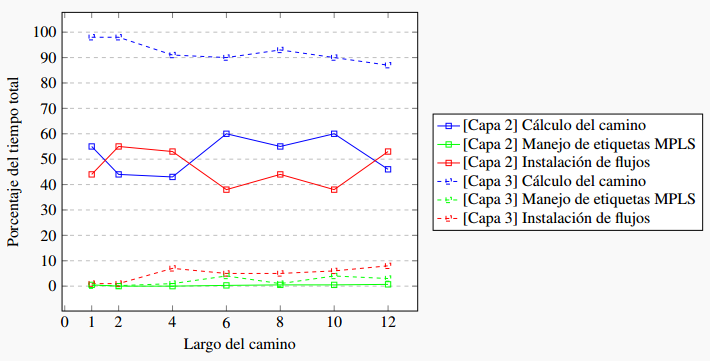
\includegraphics[scale=0.6]{porcentajes_tiempos_grande}
	\end{center}
\end{frame}

\begin{frame}{Pruebas de escala: servicios}
	Podemos analizar la escalabilidad desde dos frentes:
	\begin{enumerate}
		\item {\color{gray}\textbf{Variable}: Tamaño de la topología \\
		\textbf{Analizar}: Creación de los servicios}
		\item {\textbf{Variable}: Nivel de carga \\
		\textbf{Analizar}: Rendimiento de la red \\}
	\end{enumerate}
	\pause
	Lo ideal sería tener \textbf{modelos de tráfico}, pero no están disponibles. \\
	\pause
	Pero sí podemos crear \textbf{muchos servicios} y ver que efecto genera.
\end{frame}

\begin{frame}{Cantidad de servicios - throughput}
	\textbf{Primer enfoque}: determinar si la cantidad de servicios afecta a los RAUSwitch de forma individual (flujos).
	\pause
	\begin{center}
		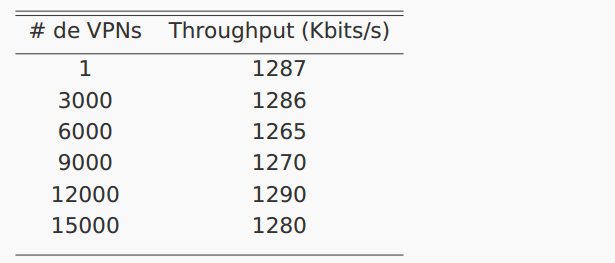
\includegraphics[scale=0.6]{throughput1}
	\end{center}
	\pause
	15.000 VPN = 1.260.000 flujos
\end{frame}

\begin{frame}{Cantidad de servicios - throughput}
	\textbf{Primer enfoque}: determinar si la cantidad de servicios afecta a los RAUSwitch de forma individual (flujos).
	\begin{center}
		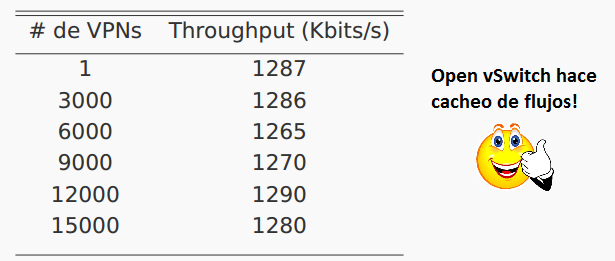
\includegraphics[scale=0.6]{throughput2}
	\end{center}
	15.000 VPN = 1.260.000 flujos
\end{frame}

\begin{frame}{Cantidad de servicios - Memoria}
	\textbf{Segundo enfoque}: consumo de memoria de RAUFlow.
	\pause
	\begin{center}
		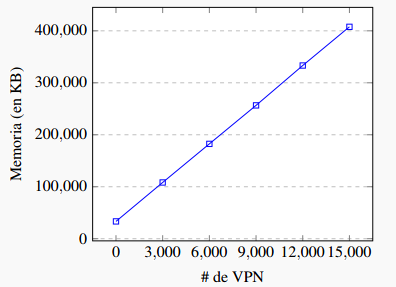
\includegraphics[scale=0.8]{memoria_rauflow}
	\end{center}
	\pause
	No es un consumo ineficiente, pero es deseable que se implemente persistencia.
\end{frame}

\begin{frame}{Cantidad de servicios - nuevo servicio}
	\textbf{Efecto inesperado}: efecto sobre la creación de nuevos servicios.
	\pause
	\begin{center}
		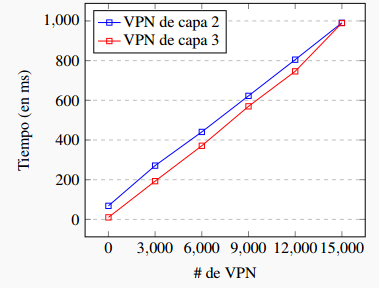
\includegraphics[scale=0.7]{cummulative_vpn}
	\end{center}
	\pause
	Falta determinar porqué ocurre (probablemente esté relacionado al consumo de memoria).
\end{frame}

%Utiliza las mismas herramientas que el prototipo físico, lo cual mejora la calidad de los experimentos. También implica que podría utilizarse en conjunto con dispositivos físicos.

\section{Conclusiones}

\begin{frame}{}
	\tableofcontents[currentsection]
\end{frame}

\begin{frame}{Conclusiones}
	\begin{itemize}
		\item Se construyó una herramienta capaz de emular arquitecturas híbridas legacy/SDN. Permite investigación sobre esquemas híbridos en general.
		\pause
		\item Se corrigieron errores de implementación en RAUFlow, y se detectaron posibles problemas que podrían afectar un despliegue real.
		\pause
		\item Se hizo un cambio en la arquitectura de RAUFlow (eliminación de SNMP), que reduce su complejidad y aumenta su rendimiento.
		\pause
		\item Se hizo un análisis de escalabilidad sobre RAUFlow, estudiando su comportamiento ante dos variables: topologias y servicios.
	\end{itemize}
\end{frame}

\begin{frame}{Conclusiones (2)}
	\begin{itemize}
		\item Se contribuyó a un artículo científico que fue aceptado en la conferencia ACM SIGCOMM Workshop on Fostering Latin American Research in Data Communication Networks (LANCOMM 2016).
		\item El artículo también fue aceptado en formato de póster en la conferencia Spring School on Networks (SSN 2016) a llevarse a cabo en Chile.
	\end{itemize}
\end{frame}

\begin{frame}{Trabajo futuro}
	Sobre el emulador y las pruebas:
	\begin{itemize}
		\item Agregarle una interfaz gráfica para que sea más fácil de usar (MiniEdit).
		\pause
		\item Explorar a fondo algunos comportamientos detectados (por ejemplo, el efecto acumulativo en la creación de VPNs).
		\pause
		\item Hacer pruebas más realistas, con modelos de tráfico que reflejen la actividad de la RAU.
	\end{itemize}
\end{frame}

\begin{frame}{Trabajo futuro}
	Sobre RAUFlow:
	\begin{itemize}
		\item Mejorar la implementación de VPN (diferentes caminos, load balancing, ingeniería de tráfico)
		\pause
		\item Implementar nuevas funcionalidades de acuerdo a los requerimientos de la RAU.
		\pause
		\item Implementar persistencia, para que no tenga todos los datos en memoria.
	\end{itemize}
\end{frame}

\begin{frame}{}
	\begin{center}
		{\huge ¿Preguntas?}
	\end{center}
\end{frame}

\end{document}

